\documentclass{article}\usepackage{graphicx, color}
%% maxwidth is the original width if it is less than linewidth
%% otherwise use linewidth (to make sure the graphics do not exceed the margin)
\makeatletter
\def\maxwidth{ %
  \ifdim\Gin@nat@width>\linewidth
    \linewidth
  \else
    \Gin@nat@width
  \fi
}
\makeatother

\IfFileExists{upquote.sty}{\usepackage{upquote}}{}
\definecolor{fgcolor}{rgb}{0.2, 0.2, 0.2}
\newcommand{\hlnumber}[1]{\textcolor[rgb]{0,0,0}{#1}}%
\newcommand{\hlfunctioncall}[1]{\textcolor[rgb]{0.501960784313725,0,0.329411764705882}{\textbf{#1}}}%
\newcommand{\hlstring}[1]{\textcolor[rgb]{0.6,0.6,1}{#1}}%
\newcommand{\hlkeyword}[1]{\textcolor[rgb]{0,0,0}{\textbf{#1}}}%
\newcommand{\hlargument}[1]{\textcolor[rgb]{0.690196078431373,0.250980392156863,0.0196078431372549}{#1}}%
\newcommand{\hlcomment}[1]{\textcolor[rgb]{0.180392156862745,0.6,0.341176470588235}{#1}}%
\newcommand{\hlroxygencomment}[1]{\textcolor[rgb]{0.43921568627451,0.47843137254902,0.701960784313725}{#1}}%
\newcommand{\hlformalargs}[1]{\textcolor[rgb]{0.690196078431373,0.250980392156863,0.0196078431372549}{#1}}%
\newcommand{\hleqformalargs}[1]{\textcolor[rgb]{0.690196078431373,0.250980392156863,0.0196078431372549}{#1}}%
\newcommand{\hlassignement}[1]{\textcolor[rgb]{0,0,0}{\textbf{#1}}}%
\newcommand{\hlpackage}[1]{\textcolor[rgb]{0.588235294117647,0.709803921568627,0.145098039215686}{#1}}%
\newcommand{\hlslot}[1]{\textit{#1}}%
\newcommand{\hlsymbol}[1]{\textcolor[rgb]{0,0,0}{#1}}%
\newcommand{\hlprompt}[1]{\textcolor[rgb]{0.2,0.2,0.2}{#1}}%

\usepackage{framed}
\makeatletter
\newenvironment{kframe}{%
 \def\at@end@of@kframe{}%
 \ifinner\ifhmode%
  \def\at@end@of@kframe{\end{minipage}}%
  \begin{minipage}{\columnwidth}%
 \fi\fi%
 \def\FrameCommand##1{\hskip\@totalleftmargin \hskip-\fboxsep
 \colorbox{shadecolor}{##1}\hskip-\fboxsep
     % There is no \\@totalrightmargin, so:
     \hskip-\linewidth \hskip-\@totalleftmargin \hskip\columnwidth}%
 \MakeFramed {\advance\hsize-\width
   \@totalleftmargin\z@ \linewidth\hsize
   \@setminipage}}%
 {\par\unskip\endMakeFramed%
 \at@end@of@kframe}
\makeatother

\definecolor{shadecolor}{rgb}{.97, .97, .97}
\definecolor{messagecolor}{rgb}{0, 0, 0}
\definecolor{warningcolor}{rgb}{1, 0, 1}
\definecolor{errorcolor}{rgb}{1, 0, 0}
\newenvironment{knitrout}{}{} % an empty environment to be redefined in TeX

\usepackage{alltt}
\usepackage[sc]{mathpazo}
\usepackage{geometry}
\geometry{verbose,tmargin=2.5cm,bmargin=2.5cm,lmargin=2.5cm,rmargin=2.5cm}
\setcounter{secnumdepth}{2}
\setcounter{tocdepth}{2}
\usepackage{url}
\usepackage[unicode=true,pdfusetitle, bookmarks=true,bookmarksnumbered=true,bookmarksopen=true,bookmarksopenlevel=2, breaklinks=false,pdfborder={0 0 1},backref=false,colorlinks=false] {hyperref}
\hypersetup{ pdfstartview={XYZ null null 1}}
\usepackage{breakurl}
\parindent = 0pt
\usepackage{amsfonts}
\usepackage{amsmath}
\usepackage{framed, color}
\definecolor{shadecolor}{RGB}{211, 211, 211}

\def\be{\begin{enumerate}}
\def\ee{\end{enumerate}}
\def\vh{\vskip0mm\hskip9mm}
\def\vn{\vskip0mm}
\def\vvn{\vskip0mm\noindent}
\def\vnn{\vskip0mm\noindent}
\def\h{\hskip4mm}
\def\bul{$\bullet$}
\def\P{\mathrm{Pr}}
\begin{document}



\begin{center}
{\bf MIKE LEDERLE\\ STATISTICS 641 - ASSIGNMENT \#4 - NOON (CDT) Friday - 10/5/2012}
\end{center}
\vskip0mm\noindent
\normalsize
\vnn\vnn
$\bullet$ Read Handouts 6 \& 7 and  Chapters 2 \& 4 in the Textbook.
\vnn\vnn
$\bullet$ Submit for grading the following problems:
\vnn\vnn
I.\ ( 45 points)\ \ A researcher is studying the relative brain weights (brain weight divided by body weight) for 51 species of mammal whose average litter size is less than 2 and for 45 species of mammal whose average litter size is greater than or equal to 2. The researcher was interested in determining what evidence that brain sizes tend to be different for the two groups. (Data from {\it The Statistical Sleuth} by Fred Ramsey and Daniel Schafer).
  \vvn
  \begin{verbatim}
                   RELATIVE BRAIN WEIGHTS - SMALL LITTER SIZE

   0.42    0.86    0.88    1.11    1.34    1.38    1.42    1.47    1.63
   1.73    2.17    2.42    2.48    2.74    2.74    2.79    2.90    3.12
   3.18    3.27    3.30    3.61    3.63    4.13    4.40    5.00    5.20
   5.59    7.04    7.15    7.25    7.75    8.00    8.84    9.30    9.68
   10.32   10.41   10.48   11.29   12.30   12.53   12.69   14.14   14.15
   14.27   14.56   15.84   18.55   19.73   20.00

                   RELATIVE BRAIN WEIGHTS - LARGE LITTER SIZE

    0.94    1.26    1.44    1.49    1.63    1.80    2.00    2.00    2.56
    2.58    3.24    3.39    3.53    3.77    4.36    4.41    4.60    4.67
    5.39    6.25    7.02    7.89    7.97    8.00    8.28    8.83    8.91
    8.96    9.92   11.36   12.15   14.40   16.00   18.61   18.75   19.05
   21.00   21.41   23.27   24.71   25.00   28.75   30.23   35.45   36.35
  \end{verbatim}
\vvn
\be
\item[1.] For the Large Litter Size mammals, Compute a 10\% trimmed mean, and compare it to the untrimmed sample mean. Does this comparison suggest any extreme values in the data?
\begin{shaded}
\begin{knitrout}
\definecolor{shadecolor}{rgb}{0.969, 0.969, 0.969}\color{fgcolor}\begin{kframe}
\begin{alltt}
large <- \hlfunctioncall{c}(0.94, 1.26, 1.44, 1.49, 1.63, 1.8, 2, 2, 2.56, 2.58, 3.24, 3.39, 3.53, 3.77, 4.36, 
    4.41, 4.6, 4.67, 5.39, 6.25, 7.02, 7.89, 7.97, 8, 8.28, 8.83, 8.91, 8.96, 9.92, 11.36, 
    12.15, 14.4, 16, 18.61, 18.75, 19.05, 21, 21.41, 23.27, 24.71, 25, 28.75, 30.23, 35.45, 
    36.35)
\hlfunctioncall{mean}(large, 0.1)
\end{alltt}
\begin{verbatim}
## [1] 9.667
\end{verbatim}
\begin{alltt}
\hlfunctioncall{mean}(large)
\end{alltt}
\begin{verbatim}
## [1] 10.97
\end{verbatim}
\end{kframe}
\end{knitrout}

Yes, it suggests there are extreme values, since when we remove the tails,
we get a value different (12\% different) than the untrimmed mean.
\end{shaded}
\item[2.] The researcher suggested a Weibull distribution to model the data for the Large Litter Size mammals. Assuming that the Weibull distribution is an appropriate model for the Large Litter Size data, obtain the MLE estimates of the Weibull parameters for the Large Litter Size data.
\begin{shaded}
Can calculate via {\tt MASS} library (as given in notes):
\begin{knitrout}
\definecolor{shadecolor}{rgb}{0.969, 0.969, 0.969}\color{fgcolor}\begin{kframe}
\begin{alltt}
\hlfunctioncall{library}(MASS)
(f <- \hlfunctioncall{fitdistr}(large, \hlstring{"weibull"}))
\end{alltt}


{\ttfamily\noindent\textcolor{warningcolor}{\#\# Warning: NaNs produced}}\begin{verbatim}
##     shape     scale 
##    1.1327   11.4982 
##  ( 0.1317) ( 1.6007)
\end{verbatim}
\begin{alltt}
\hlfunctioncall{str}(f)
\end{alltt}
\begin{verbatim}
## List of 5
##  $ estimate: Named num [1:2] 1.13 11.5
##   ..- attr(*, "names")= chr [1:2] "shape" "scale"
##  $ sd      : Named num [1:2] 0.132 1.601
##   ..- attr(*, "names")= chr [1:2] "shape" "scale"
##  $ vcov    : num [1:2, 1:2] 0.0174 0.0687 0.0687 2.5622
##   ..- attr(*, "dimnames")=List of 2
##   .. ..$ : chr [1:2] "shape" "scale"
##   .. ..$ : chr [1:2] "shape" "scale"
##  $ loglik  : num -152
##  $ n       : int 45
##  - attr(*, "class")= chr "fitdistr"
\end{verbatim}
\begin{alltt}
shape <- f$estimate[1]
scale <- f$estimate[2]
\end{alltt}
\end{kframe}
\end{knitrout}




\end{shaded}
\item[3.] Estimate the probability that a randomly selected mammal with a litter size of 5 will have a relative brain weight  greater than 30.
\begin{shaded}
\begin{knitrout}
\definecolor{shadecolor}{rgb}{0.969, 0.969, 0.969}\color{fgcolor}\begin{kframe}
\begin{alltt}
\hlfunctioncall{pweibull}(30, shape, scale, lower.tail = FALSE)
\end{alltt}
\begin{verbatim}
## [1] 0.05166
\end{verbatim}
\end{kframe}
\end{knitrout}

\end{shaded}
\item[4.] Compare the MLE estimates of $\mu$ and $\sigma$ based on the Weibull model to the distribution-free estimates of  $\mu$ and $\sigma$ for the Large Litter Size data.
\begin{shaded}
The weibull mean and standard deviation are
\begin{knitrout}
\definecolor{shadecolor}{rgb}{0.969, 0.969, 0.969}\color{fgcolor}\begin{kframe}
\begin{alltt}
mu.weibull <- scale * \hlfunctioncall{gamma}(1 + 1/shape)
\hlfunctioncall{names}(mu.weibull) <- NULL
mu.weibull
\end{alltt}
\begin{verbatim}
## [1] 10.99
\end{verbatim}
\begin{alltt}
sigma.weibull <- \hlfunctioncall{sqrt}(scale^2 * (\hlfunctioncall{gamma}(1 + 2/shape) - \hlfunctioncall{gamma}(1 + 1/shape)^2))
\hlfunctioncall{names}(sigma.weibull) <- NULL
sigma.weibull
\end{alltt}
\begin{verbatim}
## [1] 9.725
\end{verbatim}
\end{kframe}
\end{knitrout}

The distribution-free estimates are
\begin{knitrout}
\definecolor{shadecolor}{rgb}{0.969, 0.969, 0.969}\color{fgcolor}\begin{kframe}
\begin{alltt}
\hlfunctioncall{mean}(large)
\end{alltt}
\begin{verbatim}
## [1] 10.97
\end{verbatim}
\begin{alltt}
\hlfunctioncall{sd}(large)
\end{alltt}
\begin{verbatim}
## [1] 9.837
\end{verbatim}
\end{kframe}
\end{knitrout}

\end{shaded}
\item[5.] Compare the MLE estimates of median and IQR based on the Weibull model to the distribution-free estimates of  median and IQR for the Large Litter Size data.
\begin{shaded}
For the weibull model:
\begin{knitrout}
\definecolor{shadecolor}{rgb}{0.969, 0.969, 0.969}\color{fgcolor}\begin{kframe}
\begin{alltt}
first.weibull <- \hlfunctioncall{qweibull}(0.25, shape, scale)
median.weibull <- \hlfunctioncall{qweibull}(0.5, shape, scale)
third.weibull <- \hlfunctioncall{qweibull}(0.75, shape, scale)
(IQR.weibull <- third.weibull - first.weibull)
\end{alltt}
\begin{verbatim}
## [1] 11.51
\end{verbatim}
\begin{alltt}
median.weibull
\end{alltt}
\begin{verbatim}
## [1] 8.32
\end{verbatim}
\end{kframe}
\end{knitrout}

\end{shaded}
Distribution-free estimates:
\begin{shaded}
\begin{knitrout}
\definecolor{shadecolor}{rgb}{0.969, 0.969, 0.969}\color{fgcolor}\begin{kframe}
\begin{alltt}
\hlfunctioncall{IQR}(large)
\end{alltt}
\begin{verbatim}
## [1] 15.22
\end{verbatim}
\begin{alltt}
\hlfunctioncall{median}(large)
\end{alltt}
\begin{verbatim}
## [1] 7.97
\end{verbatim}
\end{kframe}
\end{knitrout}


\end{shaded}
\item[6.] Without any assumed model, estimate the mean and standard deviation of the relative brain weights for both Large and Small litter sizes.
\begin{shaded}
{\sl NOTE: I am making the assumption that we are going distribution-free
for the rest of the problem.}
\begin{knitrout}
\definecolor{shadecolor}{rgb}{0.969, 0.969, 0.969}\color{fgcolor}\begin{kframe}
\begin{alltt}
small <- \hlfunctioncall{c}(0.42, 0.86, 0.88, 1.11, 1.34, 1.38, 1.42, 1.47, 1.63, 1.73, 2.17, 2.42, 2.48, 2.74, 
    2.74, 2.79, 2.9, 3.12, 3.18, 3.27, 3.3, 3.61, 3.63, 4.13, 4.4, 5, 5.2, 5.59, 7.04, 7.15, 
    7.25, 7.75, 8, 8.84, 9.3, 9.68, 10.32, 10.41, 10.48, 11.29, 12.3, 12.53, 12.69, 14.14, 
    14.15, 14.27, 14.56, 15.84, 18.55, 19.73, 20)

\hlfunctioncall{mean}(large)
\end{alltt}
\begin{verbatim}
## [1] 10.97
\end{verbatim}
\begin{alltt}
\hlfunctioncall{mean}(small)
\end{alltt}
\begin{verbatim}
## [1] 6.886
\end{verbatim}
\begin{alltt}
\hlfunctioncall{sd}(large)
\end{alltt}
\begin{verbatim}
## [1] 9.837
\end{verbatim}
\begin{alltt}
\hlfunctioncall{sd}(small)
\end{alltt}
\begin{verbatim}
## [1] 5.46
\end{verbatim}
\end{kframe}
\end{knitrout}

\end{shaded}

\item[7.] Estimate the median and MAD of the relative brain weights for both Large and Small litter sizes.
\begin{shaded}
\begin{knitrout}
\definecolor{shadecolor}{rgb}{0.969, 0.969, 0.969}\color{fgcolor}\begin{kframe}
\begin{alltt}
MAD <- \hlfunctioncall{function}(samp) \{
    \hlfunctioncall{median}(\hlfunctioncall{abs}(samp - \hlfunctioncall{median}(samp)))/0.6745
\}

\hlfunctioncall{median}(large)
\end{alltt}
\begin{verbatim}
## [1] 7.97
\end{verbatim}
\begin{alltt}
\hlfunctioncall{MAD}(large)
\end{alltt}
\begin{verbatim}
## [1] 8.021
\end{verbatim}
\begin{alltt}
\hlfunctioncall{median}(small)
\end{alltt}
\begin{verbatim}
## [1] 5
\end{verbatim}
\begin{alltt}
\hlfunctioncall{MAD}(small)
\end{alltt}
\begin{verbatim}
## [1] 5.234
\end{verbatim}
\end{kframe}
\end{knitrout}


\end{shaded}
\item[8.] Based on your plots from Assignment \#3, which pair of estimates of the center and spread in the two data sets best represents the center and spread in the two populations of relative brain weights?
\begin{shaded}
\begin{knitrout}
\definecolor{shadecolor}{rgb}{0.969, 0.969, 0.969}\color{fgcolor}\begin{kframe}
\begin{alltt}
\hlfunctioncall{plot}(\hlfunctioncall{density}(large, window = \hlstring{"g"}, bw = \hlstring{"nrd"}), type = \hlstring{"l"}, main = \hlstring{"Large"})
\hlfunctioncall{plot}(\hlfunctioncall{density}(small, window = \hlstring{"g"}, bw = \hlstring{"nrd"}), type = \hlstring{"l"}, main = \hlstring{"Small"})
\end{alltt}
\end{kframe}

{\centering 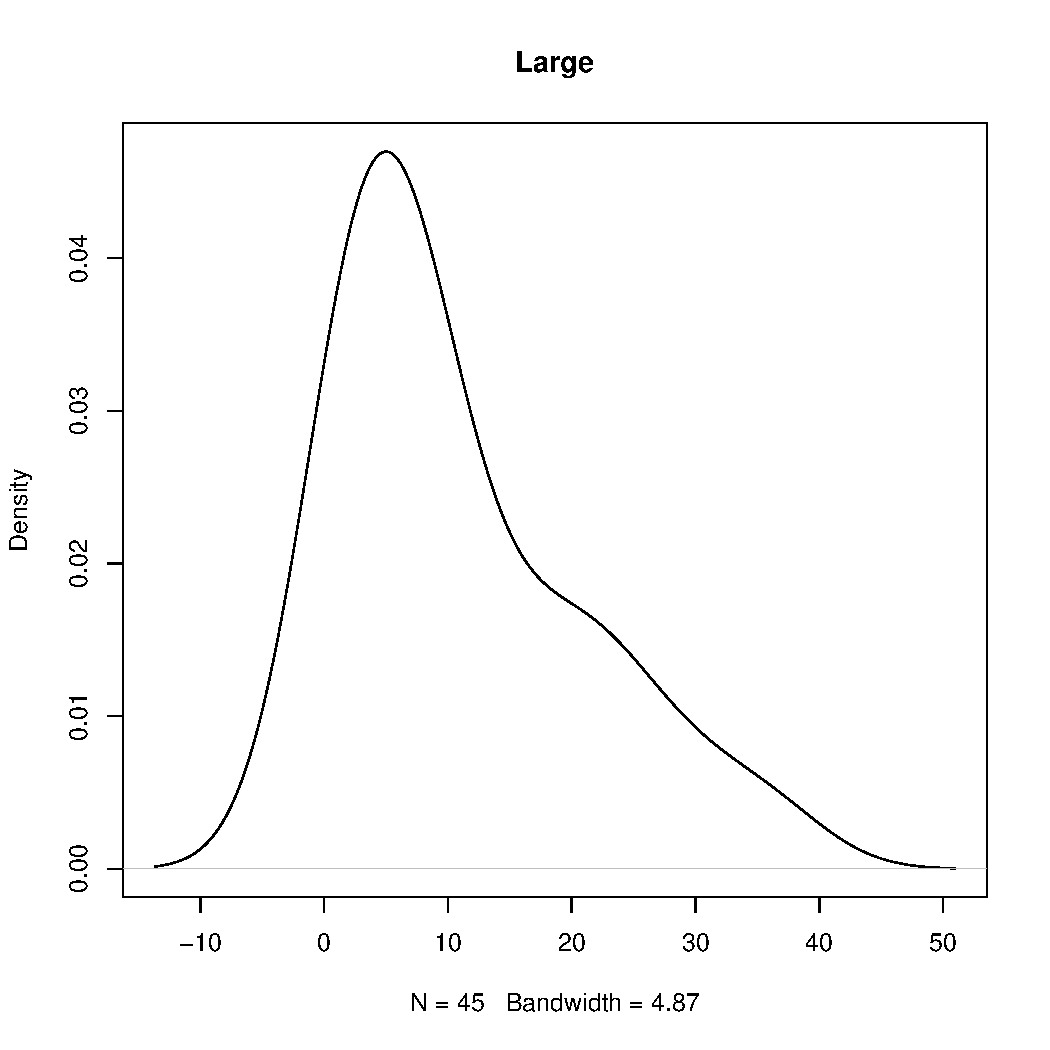
\includegraphics[width=.45\textwidth]{figure/unnamed-chunk-111} 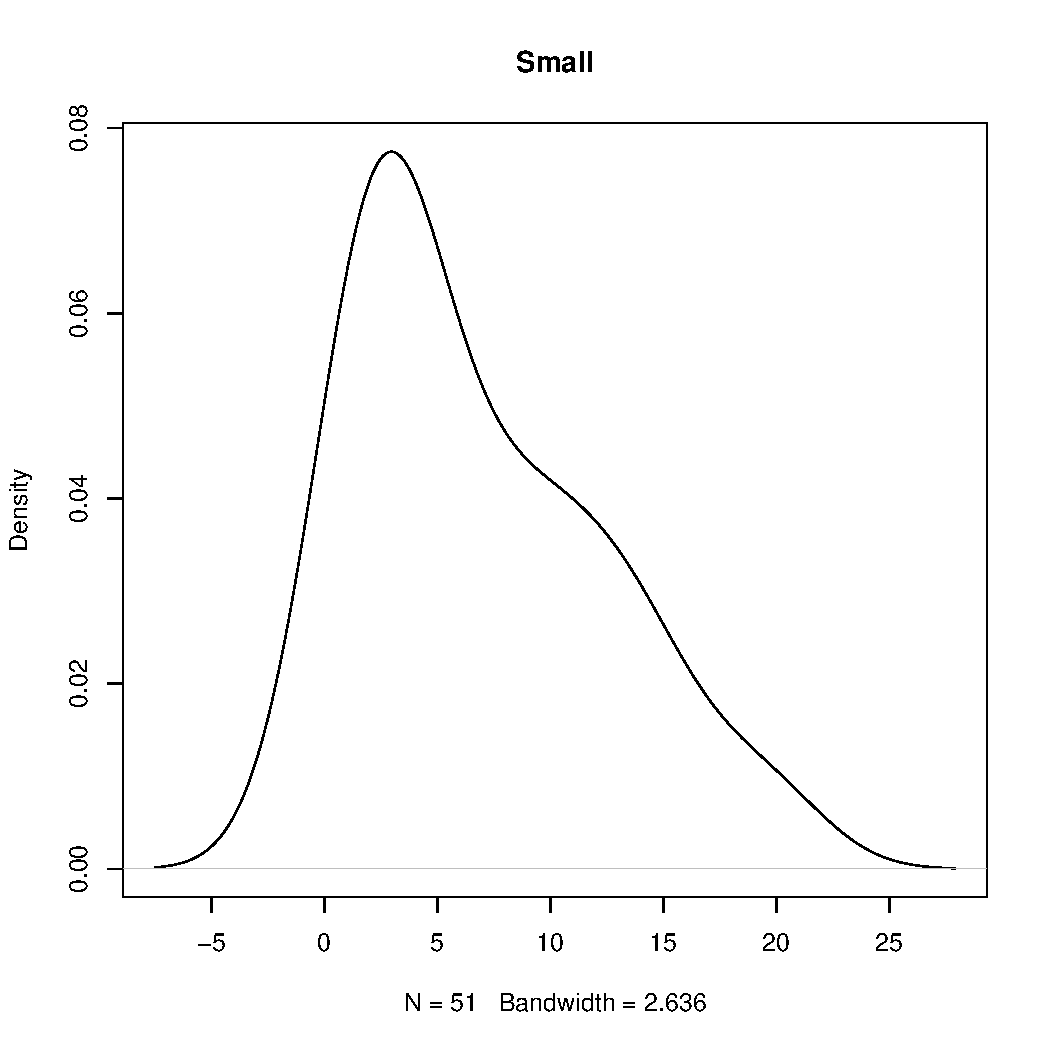
\includegraphics[width=.45\textwidth]{figure/unnamed-chunk-112} 

}


\end{knitrout}

Because the data are skewed, use the median \& MAD. 
\end{shaded}
\item[9.] Using your answers from the previous three questions, suggest a relationship (if any) between litter size and relative brain weights.
\begin{shaded}
Larger litters tend to have larger brain size.
\end{shaded}
\ee
\vvn
II.\ ( 20 points)\ \  The following data is the monthly average of daily yields of Moody's AAA bonds for the years 1989 to 1993.\\[10pt]
\vvn\vvn
\begin{tabular}{l|rrrrrrrrrrrr}
Year&Jan.&Feb.&Mar.&Apr.&May&June&July&Aug.&Sep.&Oct.&Nov.&Dec.\\\hline
1989&9.62&9.64&9.80&9.79&9.57&9.10&8.93&8.96&9.01&8.92&8.89&8.96\\
1990&8.99&9.22&9.37&9.46&9.47&9.26&9.24&9.41&9.56&9.53&9.30&9.05\\
1991&9.04&8.83&8.93&8.86&8.86&9.01&9.00&8.75&8.61&8.55&8.48&8.31\\
1992&8.20&8.29&8.35&8.33&8.28&8.22&8.07&7.95&7.92&7.99&8.10&7.98\\
1993&7.91&7.71&7.58&7.46&7.43&7.33&7.17&6.85&6.66&6.67&6.93&6.90\\
\end{tabular}\\[10pt]
\vvn
The R code {\bf Assignment04ProbII\_2012.R} provided in Files/Homework Assignments will be very useful in this problem.
\vvn
\be
\item[1.] Create a time series plot of the data.
\begin{shaded}
\begin{knitrout}
\definecolor{shadecolor}{rgb}{0.969, 0.969, 0.969}\color{fgcolor}\begin{kframe}
\begin{alltt}
bond.yield <- \hlfunctioncall{c}(9.62, 9.64, 9.8, 9.79, 9.57, 9.1, 8.93, 8.96, 9.01, 8.92, 8.89, 8.96, 8.99, 
    9.22, 9.37, 9.46, 9.47, 9.26, 9.24, 9.41, 9.56, 9.53, 9.3, 9.05, 9.04, 8.83, 8.93, 8.86, 
    8.86, 9.01, 9, 8.75, 8.61, 8.55, 8.48, 8.31, 8.2, 8.29, 8.35, 8.33, 8.28, 8.22, 8.07, 7.95, 
    7.92, 7.99, 8.1, 7.98, 7.91, 7.71, 7.58, 7.46, 7.43, 7.33, 7.17, 6.85, 6.66, 6.67, 6.93, 
    6.9)
bond.ts <- \hlfunctioncall{ts}(bond.yield, frequency = 12, start = \hlfunctioncall{c}(1989, 1))
\hlfunctioncall{plot}(bond.ts)
\end{alltt}
\end{kframe}

{\centering 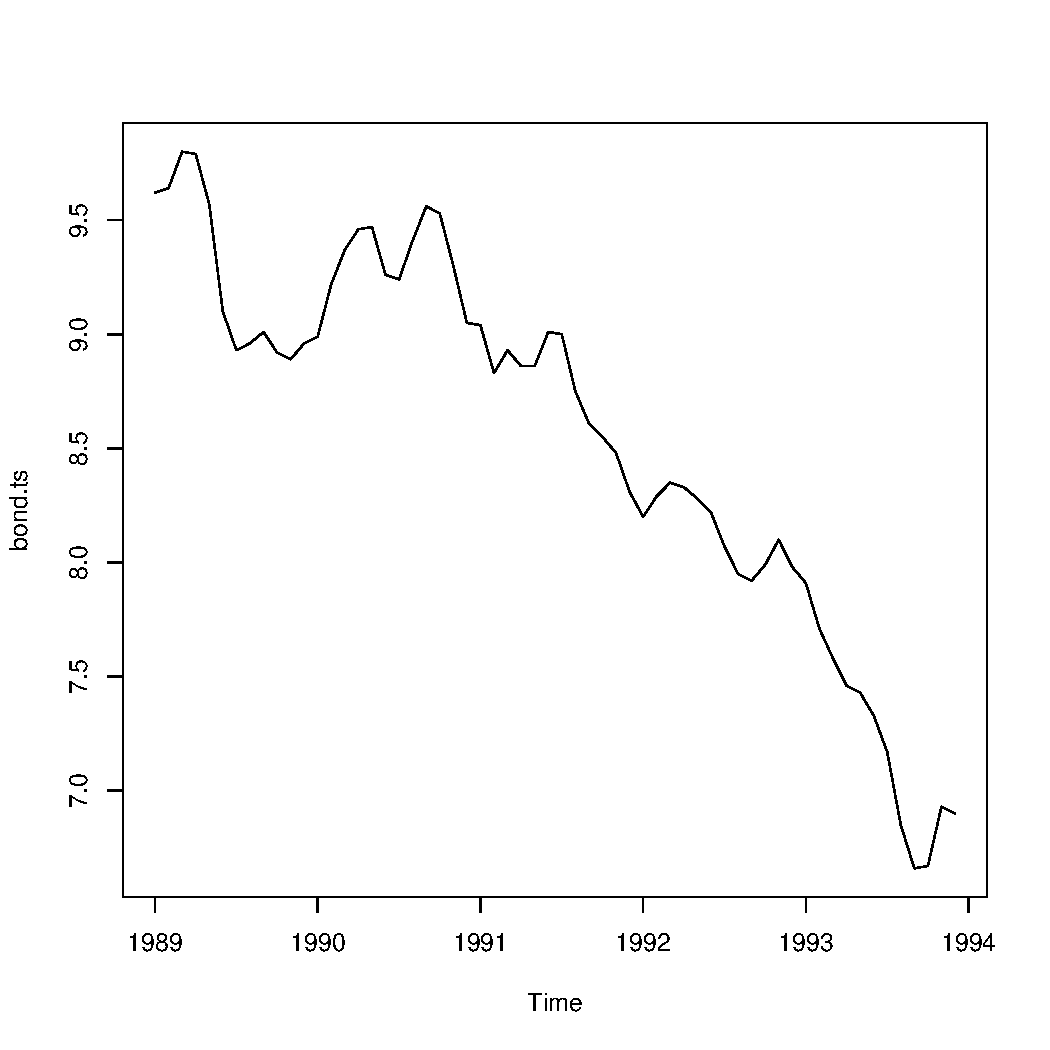
\includegraphics[width=.55\textwidth]{figure/unnamed-chunk-12} 

}


\end{knitrout}

\end{shaded}
\vfil
\newpage
\item[2.] Calculate the values of $\rho_k$, the autocorrelation coefficients.
What conclusions can you draw?
\begin{shaded}
\begin{knitrout}
\definecolor{shadecolor}{rgb}{0.969, 0.969, 0.969}\color{fgcolor}\begin{kframe}
\begin{alltt}
bond.acf <- \hlfunctioncall{acf}(bond.yield, plot = TRUE)
\hlcomment{# \hlfunctioncall{str}(bond.acf)}
bond.acf$acf
\end{alltt}
\begin{verbatim}
## , , 1
## 
##         [,1]
##  [1,] 1.0000
##  [2,] 0.9390
##  [3,] 0.8645
##  [4,] 0.7747
##  [5,] 0.6896
##  [6,] 0.6181
##  [7,] 0.5677
##  [8,] 0.5241
##  [9,] 0.4821
## [10,] 0.4385
## [11,] 0.4044
## [12,] 0.3782
## [13,] 0.3569
## [14,] 0.3334
## [15,] 0.3038
## [16,] 0.2662
## [17,] 0.2264
## [18,] 0.1866
\end{verbatim}
\end{kframe}

{\centering 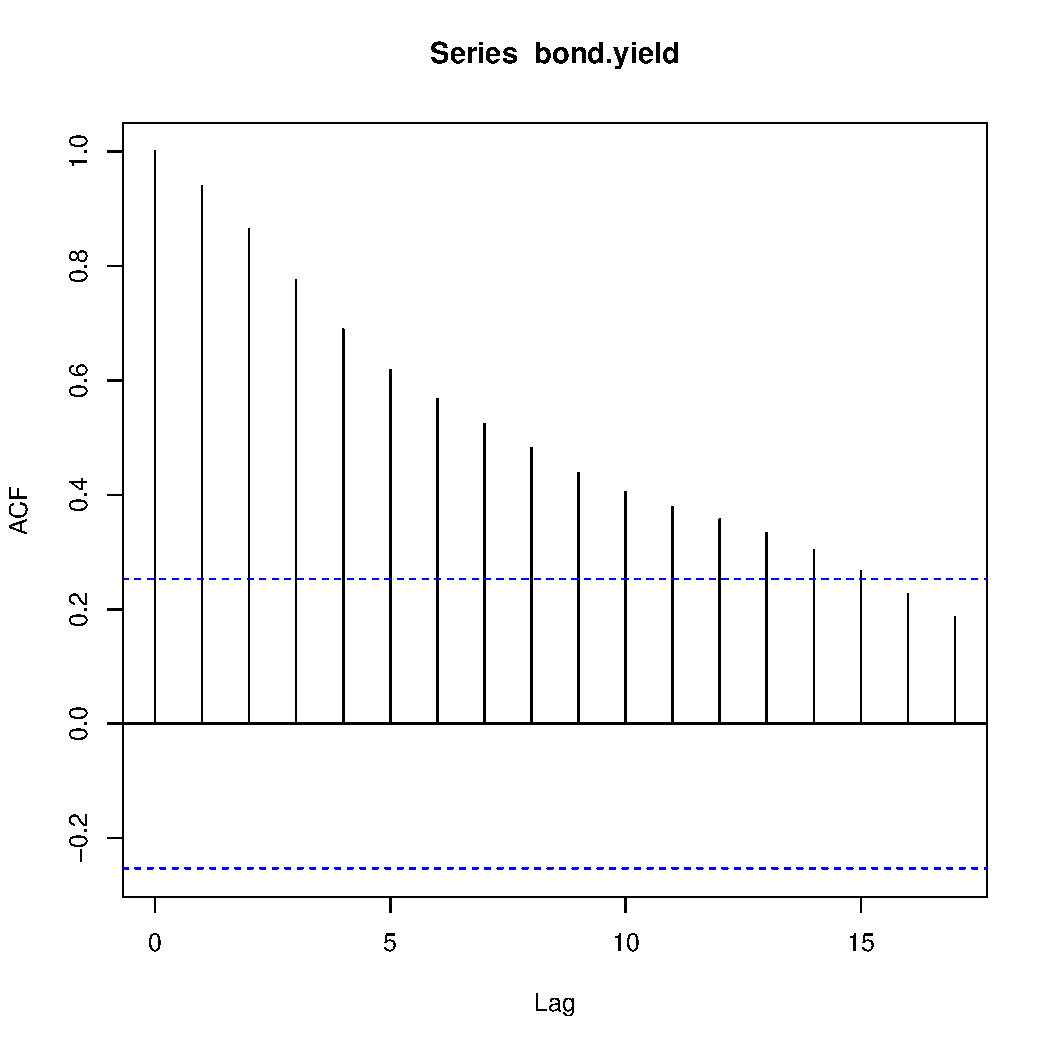
\includegraphics[width=.55\textwidth]{figure/unnamed-chunk-13} 

}


\end{knitrout}

Conclusion is strong autocorrelation, meaning the data are not random
when comparing near-adjacent values.
\end{shaded}
\item[3.] Does the time series appear to be stationary? That is, do the mean and variance
appear to remain constant over time.
\begin{shaded}
The above {\tt acf} plot indicates non-stationary behavior.
\end{shaded}
\ee
\vvn\vvn\vvn
III. (20 points)  Twenty-five patients diagnosed with rare skin disease are randomly assigned to two drug treatments. The following
times are either the time in days from the point of randomization to either a complete recovery or censoring (as indicated by
the status variable: 0 means censored, i.e., time at which patient left study prior to a complete recovery, 1 means patient's time to recovery).\\[10pt]
\vvn
\footnotesize
\begin{tabular}{l|ccccccccccccc}\hline
&\multicolumn{12}{|c}{Treatment 1}\\ \hline
Time  &180&632&2240&195&76&70&13&1990&18&700&210&1296&23\\
Status&1  &1  &1   &1  &1 &1 &0 &0   &1 &1  &1  &1   &1\\\hline\hline
&\multicolumn{12}{|c}{Treatment 2}\\ \hline
Time  &8&852&52&220&63&8&1976&1296&1460&63&1328&365\\
Status&0&1  &1 &1  &1 &1&0   &0   &1   &1 &1   &1\\\hline
\end{tabular}\\[10pt]
\normalsize
\vvn\vvn
The R code {\bf Assignment04ProbIII\_2012.R} provided in Files/Homework Assignments will be very useful in this problem.
\vvn
\be
\item[1.] Estimate the survival function for the two treatments.
\begin{shaded}
The survival function is estimated in the {\tt survival} column of the call to {\tt summary}.
\begin{knitrout}
\definecolor{shadecolor}{rgb}{0.969, 0.969, 0.969}\color{fgcolor}\begin{kframe}
\begin{alltt}
\hlfunctioncall{library}(survival)
T <- \hlfunctioncall{c}(180, 632, 2240, 195, 76, 70, 13, 1990, 18, 700, 210, 1296, 23, 8, 852, 52, 220, 63, 
    8, 1976, 1296, 1460, 63, 1328, 365)

ST <- \hlfunctioncall{c}(1, 1, 1, 1, 1, 1, 0, 0, 1, 1, 1, 1, 1, 0, 1, 1, 1, 1, 1, 0, 0, 1, 1, 1, 1)
G <- \hlfunctioncall{c}(1, 1, 1, 1, 1, 1, 1, 1, 1, 1, 1, 1, 1, 2, 2, 2, 2, 2, 2, 2, 2, 2, 2, 2, 2)
\hlcomment{# out <- \hlfunctioncall{cbind}(T,ST,G) S <- \hlfunctioncall{Surv}(T, ST) \hlfunctioncall{str}(S)}
results <- \hlfunctioncall{survfit}(\hlfunctioncall{Surv}(T, ST) ~ G)
\end{alltt}
\end{kframe}
\end{knitrout}

\end{shaded}

\begin{shaded}
\begin{knitrout}
\definecolor{shadecolor}{rgb}{0.969, 0.969, 0.969}\color{fgcolor}\begin{kframe}
\begin{alltt}
\hlfunctioncall{summary}(results)
\end{alltt}
\begin{verbatim}
## Call: survfit(formula = Surv(T, ST) ~ G)
## 
##                 G=1 
##  time n.risk n.event survival std.err lower 95% CI upper 95% CI
##    18     12       1    0.917  0.0798       0.7729        1.000
##    23     11       1    0.833  0.1076       0.6470        1.000
##    70     10       1    0.750  0.1250       0.5410        1.000
##    76      9       1    0.667  0.1361       0.4468        0.995
##   180      8       1    0.583  0.1423       0.3616        0.941
##   195      7       1    0.500  0.1443       0.2840        0.880
##   210      6       1    0.417  0.1423       0.2133        0.814
##   632      5       1    0.333  0.1361       0.1498        0.742
##   700      4       1    0.250  0.1250       0.0938        0.666
##  1296      3       1    0.167  0.1076       0.0470        0.591
##  2240      1       1    0.000     NaN           NA           NA
## 
##                 G=2 
##  time n.risk n.event survival std.err lower 95% CI upper 95% CI
##     8     12       1    0.917  0.0798       0.7729        1.000
##    52     10       1    0.825  0.1128       0.6311        1.000
##    63      9       2    0.642  0.1441       0.4132        0.996
##   220      7       1    0.550  0.1499       0.3224        0.938
##   365      6       1    0.458  0.1503       0.2410        0.872
##   852      5       1    0.367  0.1456       0.1684        0.798
##  1328      3       1    0.244  0.1392       0.0801        0.746
##  1460      2       1    0.122  0.1110       0.0206        0.724
\end{verbatim}
\end{kframe}
\end{knitrout}

 
\end{shaded}
\item[2.] Compare the mean and median time to death for the two treatments\begin{shaded}
Compare the mean and median columns below:
\begin{knitrout}
\definecolor{shadecolor}{rgb}{0.969, 0.969, 0.969}\color{fgcolor}\begin{kframe}
\begin{alltt}
\hlfunctioncall{print}(results, print.rmean = TRUE)
\end{alltt}
\begin{verbatim}
## Call: survfit(formula = Surv(T, ST) ~ G)
## 
##     records n.max n.start events *rmean *se(rmean) median 0.95LCL 0.95UCL
## G=1      13    13      13     11    635        216    202      76      NA
## G=2      12    12      12      9    747        226    365      63      NA
##     * restricted mean with upper limit =  2108
\end{verbatim}
\end{kframe}
\end{knitrout}

\end{shaded}
\item[3.] Which treatment appears to be most effective in the treatment of the skin disease?
\begin{shaded}
Treatment 1; both the mean and median time to recovery are less.
\end{shaded}
\ee
\vvn\vvn\vvn
IV.\ \  (15 points) {\bf Select} the letter of the {\bf BEST} answer. Justify your answer with at most 20 words.
\vskip2mm
\noindent
\small
\be
\item[1.] An experiment involves putting specimens of steel under stress until the specimen fractures. The machine increases the
stress until the specimen fractures. The maximum stress that the machine can place on a specimen is 500 psi. Out of
the 35 specimens used in the experiment, 5 did not fracture at 500 psi. This type of censoring is called
\be
\item[A.] Random censoring
\begin{shaded}
\item[B.] Type I censoring\\[5pt]
{\sl Stress force replaces time; any greater than 500 are censored.}
\end{shaded}
\item[C.] Type II censoring
\item[D.] Left censoring
\item[E.] Right censoring
\ee
\item[2.] A veterinarian  designed a study to determine
the age at which Labrador retrievers  learned how to swim. There was three groups of puppies:
\be
\item[] Group I: Puppies who knew how to swim prior to the beginning of the study;
\item[] Group II: Puppies who learned how to swim during the study;
\item[] Group III: Puppies who had not yet learned how to swim at the conclusion of the study.
\ee
The age at which each puppy learned how to swim was recorded. The values recorded for the
Group I puppies are
\be
\item[A.] Type I censored
\item[B.] Type II censored
\item[C.] Random censored
\begin{shaded}
\item[D.] Left censored\\[5pt]
{\sl Only have upper bound on the age at which swimming was learned.}
\end{shaded}
\item[E.] Uncensored
\ee
\item[3.]  Refer to Problem 2. The values recorded for the
Group II puppies are
\be
\item[A.] Type I censored
\item[B.] Type II censored
\item[C.] Random censored
\item[D.] Left censored
\begin{shaded}
\item[E.] Uncensored\\[5pt]
{\sl Complete data set.}
\end{shaded}
\ee
\item[4.]  Refer to Problem 2. The values recorded for the
Group III puppies are
\be
\begin{shaded}
\item[A.] Type I censored\\[5pt]
{\sl The study ended at $t$; only know that group III has $T > t.$}
\end{shaded}
\item[B.] Type II censored
\item[C.] Random censored
\item[D.] Left censored
\item[E.] Uncensored
\ee
\item[5.]  An engineer for an automotive manufacturer  is
studying the occurrence of a defective in the braking system for a newly designed braking system. She randomly selects 100
automobiles for study and plans to record the distance traveled prior to a failure in the braking system. However, she
needs to conclude the study 12 months after its inception. For each of the 100 automobiles she recorded the
mileage at which a failure occurred in the braking system or the mileage driven during the 12 month study for those
automobiles that did not have a failure. We would describe the data from this type of study as having
\be
\begin{shaded}
\item[A.] Type I censoring\\[5pt]
{\sl We only know lower bound on those systems that didn't fail at the study completion.}
\end{shaded}
\item[B.] Type II censoring
\item[C.] Random censoring
\item[D.] Left censoring
\item[E.] Right censoring
\ee\ee
\vvn\vvn\vvn
V.\ \ Bonus Problem for 5 points (attempt this problem only if you have extra time).
\vvn
\be
\item[]Prove the following statement:
\vnn
\item[] If $Y$ has a symmetric distribution with $\mu<\infty$ and median $\tilde{\mu}$,
\vskip2mm
then, the median of $W = |Y-\tilde{\mu}|$, equals the SIQR of $Y$.
\ee
\vfill

\end{document}
